\documentclass[10pt]{exam}
\usepackage[hon]{template-for-exam}
\usepackage{enumitem}
\usepackage{tikz}
\usepackage{multicol}
\usetikzlibrary{shadings,decorations.pathmorphing,arrows.meta}



\def\mytitle{Chapter 3 (Two-Dimensional Kinematics)}
\author{Rohrbach}
\date{\today}

\def\mymaketitle{
  \begin{flushleft}
    {\LARGE \textbf \mytitle \par}
  \end{flushleft}
}

\newcommand{\printeqs}{
  \section*{Equations} 

  \hrule
  
  \begin{minipage}{1.5in}
    \begin{center}
      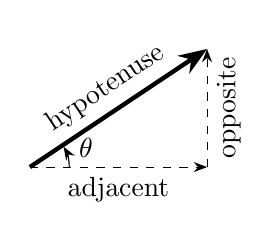
\begin{tikzpicture}[
        every node/.append style={},
        component/.append style={
          dashed,
          -{Stealth}
        },
        resultant/.append style={
          ultra thick,
          -{Stealth}
        },
        scale=0.5
    ]
      \draw[resultant] 
                (0,0) -- (4.5,3) 
                  node[midway,anchor=south,rotate=33.7]{hypotenuse};
      \draw[component] 
                (0,0) 
                -- (4.5,0) 
                  node[midway,anchor=north]{adjacent} ;
      \draw[component] 
                (4.5,0)
                -- (4.5,3) 
                  node[midway,anchor=north,rotate=90]{opposite} ;
      \draw[-Stealth] (1,0) node[anchor=south west]{$\theta$}
                arc[
                  start angle = 0,
                  end angle = 31, 
                  radius = 1
                ];
    \end{tikzpicture}


    \end{center}
  \end{minipage}
  %
  \begin{minipage}{4.9in}
    \begin{center}
      \begin{align*}
        \sin{\theta} & =\frac{\text{opp}}{\text{hyp}} &
        \cos{\theta} & =\frac{\text{adj}}{\text{hyp}} &
        \tan{\theta} & =\frac{\text{opp}}{\text{adj}}
      \end{align*}

      \hrule 
      
      \begin{align*}
        R &= \frac{v_0^{\,2} \sin\left(2\theta\right)}{g}
      \end{align*}
      
    \end{center}
  \end{minipage}


  \vspace{1em}
  \hrule
  \vspace{-.5em}
  \begin{multicols}{3}
    \begin{center}

      $v_f = v_i + a t$
    
      \emph{\footnotesize ``Old Faithful''}
    
    
      $d = v_i t + \frac{1}{2} a t^2$
    
      \emph{\footnotesize``The Big Chalupa''}
    

      $v_f^2 = v_i^2 + 2 a d$

      \emph{\footnotesize ``Ain't Got No Time''}

    \end{center}
  \end{multicols}
  \vspace{-8pt}
  \hrule
}

\begin{document}


\mymaketitle



\newcommand{\stampbox}[1]{

  \hfill
  \begin{tikzpicture}[every text node part/.style={align=center}]
     \node[gray!50,draw,rounded corners] at (0,0) 
      {\sc Stamp \\ \sc Here \\ \small #1 \sc Points};
  \end{tikzpicture}
  \vspace{1em}
  
  \hrule

}

\section*{Homework Check A (collected Fri, Sept 9)}


%%%%%%%%%%%


\paragraph{Graphical Vector Addition } p. 68 \#1, 2 
\dotfill Complete by Tue, Sept 6

{\sc Draw the pictures only; you do not need to do any calculations.}

\stampbox{2}


%%%%%%%%%%%

\paragraph{Vector Addition Calculations} pp. 68-69 \#3, 6, 8, 9, 11, 12a, 13a
\dotfill Complete by Tue, Sept 6

{\sc Must include vector diagrams showing the graphical addition and the calculations}

\stampbox{8}

%%%%%%%%%%%%

\paragraph{Projectile Motion Intro} pp. 69-70 \#17, 20, 22 
\dotfill Complete by Thu, Aug 11

{\sc Must include pictures with axes indicated}
\hfill \textbf{\emph{Homework Quiz}}


\stampbox{5}
  

%%%%%%%%%%%%%

\subsection*{Answers}

\begin{multicols}{3}

  \begin{itemize}[noitemsep]
    \item[3.] 11.7 units @ 33.1$^\circ$ S of E
    \item[6.]  $v_{1x} = -6.6$;  $v_{1y} = 0$; \\
       $v_{2x} = 4.88$;   $v_{2y} = 6.96$; \\
       7.17 units @ 76.1$^\circ$ N of W
    \item[8.] 625.4 km/h northerly; \\
       553.3 km/h westerly; \\
       1094 km North; \\
       968 km West
    \item[9.] $R_x = 24.0$;  $R_y = 11.7$;  \\
       $\vec{R} = 26.7$ units @ 26$^\circ$ N of E
    \item[11.] 64.6 units @ 53.1$^\circ$ N of E
    \item[12.] (a) 137.2 @ 73.0$^\circ$ W of S
    \item[13.] (a) 62.6 @ 58.9$^\circ$ E of S
    \item[17.] 3.71 m
    \item[20.] 7.7 m/s
    
  \end{itemize}
  
\end{multicols}

\noindent
{\footnotesize Homework will be accepted for full credit until the test.
Homework turned in after the test will be accepted for half credit
until the Unit 3 Test.
\emph{Please remember that you will not be eligible to complete 
test corrections if you do not turn in your homework.}}

\vspace{1em}
\hrule 
\printeqs


%%%%%%%%%%%%%
%%%%%%%%%%%%%

\pagebreak

\mymaketitle

\section*{Homework Check B (collected on Test Day)}

\paragraph{Projectile Motion (Involved)} pp. 69-70, 72 \#23, 26, 27, 28, 29, 55, 56, 67
\dotfill Complete by Tue, Sept 13
   
{\sc Must include pictures with axes indicated}


\stampbox{10}

%%%%%%%%%%%%%%

\paragraph{Relative Velocity} pp. 70-71 \#38, 39, 41
\dotfill Complete by Mon, Sept 19
   
\stampbox{5}

%%%%%%%%%%%%%%

\paragraph{Conceptual Questions} p. 67 \#1, 2, 4, 6, 7, 8, 9, 12, 13 ,15 17, 19
\dotfill Complete by Mon, Sept 19
   
{\sc These questions should have at least one full sentence 
      of explanation}

\stampbox{5}

%%%%%%%%%%%%%%

\paragraph{Misconceptual Questions} pp. 67-68 \#1, 2, 4, 5, 6, 8, 9, 11, 12
\dotfill Complete by Mon, Sept 19.
   
{\sc You do not need to get this one stamped,
but these are good review for your test!}

\vspace{1em}
\hrule

%%%%%%%%%%%%%%

\paragraph{Bonus Problems!} p. 69 \#19; p. 70 \#37; p. 71 \#44 \& 45
\dotfill Turn in separately on test day!

\vspace{1em}
\hrule


%%%%%%%%%%%%%%

\paragraph{Test will be on Tuesday, Sept 20.} \hfill


\subsection*{Problem Answers}

\begin{multicols}{3}

  \begin{itemize}[noitemsep]
    \item[23.] 17.7$^\circ$ \& 72.3$^\circ$
    \item[26.] 12.5 s; 50 m
    \item[27.] (a) 30.9 m;		(b) 5.02 s; \\
      (c) 136.1 m;	(d) 28.9 m/s
    \item[28.] 9.72 m/s;   8.60 m
    \item[29.] 22.3 m
    \item[55.] 0.88 s;  0.95 m
    \item[56.] 6.65 m/s
    \item[67.] 53.7$^\circ$
    \item[38.] 10.5 m/s;   6.5 ms
    \item[39.] 1.66 m/s @ 65.0$^\circ$ E of N
    \item[41.]  23.1 sec
    
    
  \end{itemize}
  
\end{multicols}

\subsection*{Misconceptual Answers}

\begin{multicols}{9}

  \begin{itemize}[noitemsep]
    \item[1.] c	
    \item[2.] a	
    \item[4.] a	
    \item[5.] b	
    \item[6.] b	
    \item[8.] d	
    \item[9.] c	
    \item[11.] b\&e	
    \item[12.] a
  \end{itemize}
  
\end{multicols}

\hrule
\vspace{0.2em}
\hrule

%%%%%%%%%%%%%%

\section*{Extra Practice}

These problems are not required and are not for bonus.  Work and answers are available on Schoology.
  
Vector Addition \dotfill \#4, 10, 12bc, 13bc

Projectile Motion \dotfill \#18, 21, 31

Relative Velocity \dotfill \#46

\end{document}